\chapter{Проектирование рентгенооптических трактов Центра коллективного пользования <<Сибирский кольцевой источник фотонов>>}\label{chap:opt_schemes}

\section{Введение к главе}
В данной главе мы рассмотрим схемы рентгенооптических трактов эксперементальных станций первой очереди ЦКП <<СКИФ>>: от источников высокоэнергетических фотонов (вставных устройств) до деталей оптических компонентов на эксперементальных станциях: фильтров, монохроматоров, бимсплитеров, рентгеновских зеркал и линз. В главе, будут обсуждаться станции: 1-1 --- <<Микрофокус>>, 1-2 --- <<Структурная диагностика>>, 1-4 --- <<XAFS-спектроскопия и магнитный дихроизм>>.

\begin{table}[h!]
	\caption{Параметры накопительного кольца и электронного пучка в ондуляторном прямом промежутке}
	\centering
	\label{table:ebeam}
	\begin{tabular}{c|c|c|c}
		\hline\hline
		%\toprule
		\rule{0pt}{3ex}   $\sigma_x, [\textup{м}]$ & $\sigma_{x'}, [\textup{рад}]$ & $\sigma_y, [\textup{м}]$     & $\sigma_{y'}, [\textup{рад}]$ \\ \hline
		\rule{0pt}{3ex}   $33,0 \times 10^{-6}$  & $2,65 \times 10^{-6}$  &  $8,6 \times 10^{-7}$ & $5,0 \times 10^{-7}$   \\
		\hline	\hline
		\rule{0pt}{3ex}   $\Delta E / E$ & $\beta_x,[\textup{м}]$ & $\beta_y,[\textup{м}]$   & $I,[\textup{мА}]$\\ \hline
		\rule{0pt}{3ex}	 $8,6 \times 10^{-4}$ & $12,49$ & $1,99$ & $400$ \\ \hline\hline
		%\toprule
	\end{tabular}
	\vspace{4pt} 
\end{table}

На этих станциях предполагается использовать излучение из сверхпроводящих ондуляторов, которые разрабатываются и будут производиться в ИЯФ СО РАН, \cite{bragin2018short} и \cite{gluskin2019superconducting}. Всё ондуляторы будут вводиться в прямой промежуток с геометрическими и угловыми размерами электронного пучка и $\beta$-функциями, указанными в таб.~\ref{table:ebeam}. 

\section{Станция 1-1 --- <<Микрофокус>>}
\subsection{Вставное устройство}
Источник излучения станции --- сверхпроводящий ондулятор с параметрами, указанными в таб.~\ref{table:und1-1}. Выбора этого типа ондулятора объясняется тем, что на станции предполагается работать на довольно высоких гармониках, поэтому, согласно рассуждениям параграфа~\ref{section:HGR} главы~\ref{chap:undulatro_radiation}, необходимо добиться как можно меньшего подавления высших гармоник. 
\begin{table}[h!]
	\caption{Параметры ондулятора для станции 1-1}
	\centering
	\begin{tabular}{c|c|c|c|c}
		\hline\hline
		\rule{0pt}{3ex}$\mathnormal{B, [\textup{Тл}]}$ & $\mathnormal{d, [\textup{мм}]}$   & $\mathnormal{K}$   & $\mathnormal{L, [\textup{м}]}$  &  Рабочие Гармоники 1-1       \\ \hline
		\rule{0pt}{3ex}$1,36$  & $18$ & $2,29$  & $2,3$         & $11, 13, 17, 23$\\
		\hline\hline
	\end{tabular}
	\label{table:und1-1}
\end{table}
На рис.~\ref{fig:log_spec_1-1} представлен спектр используемого ондулятора через конечную апертуру ($0,4$ мм), см. рис.~\ref{fig:log_spec_1-1}. Рабочие гармоники подавлены на порядок по сравнению с фундаментальной гармоникой, однако потока фотонов на этих гармониках, будет достаточно для проведения исследований на эксперементальных станциях.
\begin{figure}[h]
	\centering
	\includegraphics[width=\textwidth]{pic/log_spec_1-1.pdf}
	\caption{Спектр ондулятора с $K = 2,29$ через апертуру $0,4 \; \textup{мм}$ в логарифмическом масштабе (сверху) и в линейном (снизу), рассчитанный в коде SPECTRA с учётом эмиттанса и энергетического разброса}
	\label{fig:log_spec_1-1}
\end{figure}

\subsection{Оптика станции 1-1}\label{subsection:opt_scheme_1-1}
Первостепенной задачей по расчёту оптики станции являлась оценка тепловых нагрузок на первые оптические элементы. На рис.~\ref{fig:OptScheme_1-1} представлена оптическая схема станции, в первом приближении, без фокусирующих линз. После прохождения пучком апертуры, которая является угловым фильтром, излучение проходит алмазное окно, толщина которого $100 \; \textup{мкм}$ из расчёта $ 3 \%$ поглощения на первой рабочей гармонике. Алмазные кристаллы являются хорошими фильтрами низких энергий. Основная тепловая нагрузка с первых гармоник снимается входным алмазным окном.
\begin{figure}[h!]
	\centering  
	\includegraphics[width=\textwidth]{pic/OptScheme_1-1.pdf}
	\caption{Оптическая схема станции 1-1}
	\label{fig:OptScheme_1-1}  
\end{figure}
После алмазного окна излучение разделяется алмазными $C_d(111)$ бим-сплиттерами толщиной  $100 \; \textup{мкм}$ на рабочие секции, прямой пучок падает на кремниевый $Si(111)$ двухкристальный монохроматор. Поглощённые удельные мощности на единицу площади на оси на каждом оптическом элементе представлены найти на рис.~\ref{fig:full_spec_1-1}. 

Данные расчёты проводились следующим образом: бралось спектральное распределение электронного пучка с бесконечно малым эмиттансом, после распределение сворачивалось с кривыми поглощения соответствующих кристаллов (базу данных кривых поглощения можно найти в коде SPECTRA). Интеграл по спектру давал значение удельной мощности излучения на оси.

Полезно сравнить приведённые расчёты на рис.~\ref{fig:full_spec_1-1} с расчётами отдельного метода в коде SRW. Этот метод даёт пространственное распределения полной спектральной мощности излучения, см. рис~\ref{fig:power_dens_1-1}, который учитывает эмиттанс и конечное энергетическое распределение электронного пучка. Видно, что значения мощности излучения на оси очень близки по значению для двух расчётов: для расчётов на рис~\ref{fig:full_spec_1-1} полная удельная мощность, падающая на первый оптических элемент на оси --- $96,8 \; \textup{Вт/мм}^2$, для рис.~\ref{fig:power_dens_1-1} --- это $97,5 \; \textup{Вт/мм}^2$.

Незначительная разница объясняется тем, что во-первых, в расчётах.~\ref{fig:full_spec_1-1} не учитывался эмиттанс пучка и энергетическое распределение, что даёт переоценку значения подающей мощности, но интегрирование проводилось до значения энергии в $60 \; \textup{кэВ}$, что даёт недооценку значения мощности. В итоге, суммарно получилась недооценка, по сравнению с методом кода SRW. Подобные расчёты проводились в коде SPECTRA. Код также даёт очень близкие значения плотности мощности с приведёнными на рис.~\ref{fig:full_spec_1-1} и рис.~\ref{fig:power_dens_1-1}.

\textbf{Результаты расчётов расчётов в коде SRW для станции 1-1:}
\begin{figure}[h!]
	\centering
	\includegraphics[width=\textwidth]{pic/full_spec_1-1.pdf}
	\caption{Для станции 1-1: спектр на оси. Розовый цвет --- спектр электронного пучка с нулевым эмиттансом, падающий на алмазное окно, чёрный цвет --- спектр излучения, падающий на двукристалльный монохроматор}
	\label{fig:full_spec_1-1}   
\end{figure}
%Полезно сравнить расчёты связанные с полной падающей мощность на первый оптический элемент с одним из результатов встроенной функции в SRW по расчёту полной мощности, результаты этих расчётов приведены на рис.~\ref{fig:power_dens_1-1}. Необходимо отметить, что  эти расчёты~\ref{fig:full_spec_1-1} и рис.~\ref{fig:power_dens_1-1} независимы и совпадают, а незначительное отличие заключается лишь в том, что интегрирование на рис.~\ref{fig:full_spec_1-1} велось не по полному спектру, а лишь до энергии $60 \; \textup{кэВ}$, что не может привести ошибкам в расчётах, так как были не учтены фотоны с энергиями больше $60 \; \textup{кэВ}$, однако они являются прозрачными для большинства оптических элементов и не вносят значительного вклада в тепловые нагрузки.

\DTLloaddb
[
noheader,
keys={},
headers={
	\shortstack{$n_{\textup{{\normalfont гарм}}}$},
	\shortstack{$\sigma_x, [\textup{{\normalfont мм}}]$},
	\shortstack{$\sigma_y, [\textup{{\normalfont мм}}]$},
	\shortstack{$\sigma_x, [\textup{{\normalfont мкрад}}]$},
	\shortstack{$\sigma_y, [\textup{{\normalfont мкрад}}]$}}
]
{RMS_before1-1}{tabl_1-1/RMS_before1-1.csv}
\begin{table}[h!]
	\caption{Для станции 1-1: сечение пучка на входе в первую апертуру (25 м) с учётом эмиттанса и энергетического разброса}
	\sisetup{
		parse-numbers   = false,
		table-number-alignment = right,
		table-figures-integer = 4,
		table-figures-decimal = 4,
		input-decimal-markers = .
	}
	\renewcommand*\dtlrealalign{S}
	\centering
	\DTLdisplaydb{RMS_before1-1}
	\label{table:size_obeam}
\end{table}

	\DTLloaddb
[
noheader,
keys={},
headers={
	\shortstack{$n_{\textup{{\normalfont гарм}}}$},
	\shortstack{$\theta_{ \textup{{\normalfont Б}}}, \textup{{\normalfont град}}$},
	\shortstack{$d_{\textup{{\normalfont эф}}}, \textup{{\normalfont мкм}}$},
	\shortstack{$S_{\textup{{\normalfont пр}}}, \textup{{\normalfont мм}}$}}
]
{Cr_angles1-1}{tabl_1-1/Cr_angles1-1.csv}
\begin{table}[h!]
	\caption{Для станции 1-1: номер гармоники, ориентация кристалла, эффективная толщина алмазного бим-сплиттера, проекция пучка (горизонтальная) }
	\sisetup{
		parse-numbers   = false,
		table-number-alignment = right,
		table-figures-integer = 4,
		table-figures-decimal = 4,
		input-decimal-markers = .
	}
	\renewcommand*\dtlrealalign{S}
	\centering
	\DTLdisplaydb{Cr_angles1-1}
	\label{table:stable}
\end{table}

\DTLloaddb
[
noheader,
keys={},
headers={
	\shortstack{$n_{harm}$},
	\shortstack{$\sigma_x, [\textup{{\normalfont мм}}]$},
	\shortstack{$\sigma_y, [\textup{{\normalfont мм}}]$},
	\shortstack{$\sigma_x, [\textup{{\normalfont мкрад}}]$},
	\shortstack{$\sigma_y, [\textup{{\normalfont мкрад}}]$}}
]
{RMS_after1-1}{tabl_1-1/RMS_after1-1.csv}
\begin{table}[h!]
	\caption{Для станции 1-1: сечение пучка после бим-сплиттеров и монохроматора с учётом эмиттанса и энергетического разброса}
	\sisetup{
		parse-numbers   = false,
		table-number-alignment = right,
		table-figures-integer = 4,
		table-figures-decimal = 4,
		input-decimal-markers = .
	}
	\renewcommand*\dtlrealalign{S}
	\centering
	\DTLdisplaydb{RMS_after1-1}
	\label{table:size_obeam_after}
\end{table}

\DTLloaddb
[
noheader,
keys={},
headers={
	\shortstack{$n_{\textup{{\normalfont гарм}}}$},
	\shortstack{$E, \textup{{\normalfont [эВ]}}$},
	\shortstack{$\lambda, \textup{{\normalfont [нм] }}$},
	\shortstack{$\gamma/\textup{{\normalfont с}}$},
	\shortstack{$\gamma/\textup{{\normalfont с}}/0.1\%\mathnormal{bw}$},
	\shortstack{$\Delta E / E$}}
]
{ph_beam_par_after_cr1-1}{tabl_1-1/ph_beam_par_after_cr1-1.csv}
\begin{table}[h!]
	\caption{Для станции 1-1: потоки фотонов после бим-сплиттеров и монохроматора}
	\sisetup{
		parse-numbers   = false,
		table-number-alignment = right,
		table-figures-integer = 4,
		table-figures-decimal = 4,
		input-decimal-markers = .
	}
	\renewcommand*\dtlrealalign{S}
	\centering
	\DTLdisplaydb{ph_beam_par_after_cr1-1}
\end{table}
\newpage
\section{Станция 1-2 --- <<Структурная диагностика>>}
\subsection{Вставное устройство}
Станция 1-2 основана на использовании сверхпроводящего ондулятора с параметром ондуляторности $K = 1,54$. На станции, в отличии от 1-1, предполагается работать на более низких гармониках, этим объясняется выбор указанного параметра $K$, амплитудный спектр смещён в сторону фундаментальной гармоники и сильнее подавлен на высоких гармониках. В таб.~\ref{table:und1-2} приведены основные характеристики используемого ондулятора, на рис.~\ref{fig:log_spec_1-2} показан спектр этого ондулятора через апертуру $0,4$ мм. 
\begin{table}[h!]
	\caption{Параметры ондулятора для станции 1-2}
	\centering
	\begin{tabular}{c|c|c|c|c}
		\hline\hline
		\rule{0pt}{3ex}$\mathnormal{B, [\textup{Tл}]}$   & $\mathnormal{d, [\textup{mm}]}$ & $\mathnormal{K}$   & $\mathnormal{L, [\textup{м}]}$  &  Рабочие Гармоники 1-2       \\ \hline
		\rule{0pt}{3ex}$1,06$    			  & $15,6$& $1,54$    			  & $2$                         		   & $5, 7, 9, 13$\\
		\hline\hline
	\end{tabular}
	\label{table:und1-2}
\end{table}

\begin{figure}[h!]
	\centering
	\includegraphics[width=\textwidth]{pic/log_spec_1-2.pdf}
	\caption{Спектр с ондулятора с $K = 1,54$ через апертуру $0,4 \; \textup{мм}$ в логарифмическом масштабе (сверху) и в линейном (снизу) посчитанный в коде SPECTRA с учётом эмиттанса и энергетического разброса}
	\label{fig:log_spec_1-2}
\end{figure}

\subsection{Оптика станции 1-2}
Оптическая схема станции, с точки зрения расчётов, аналогична станции 1-1, с одним лишь отличием в том, что используется другой тип ондулятора и более низкие рабочие гармоники. На рис.~\ref{fig:OptScheme_1-2} приведена схема станции, совпадающая по структуре со схемой для 1-1. 
\begin{figure}[h!]
	\centering  
	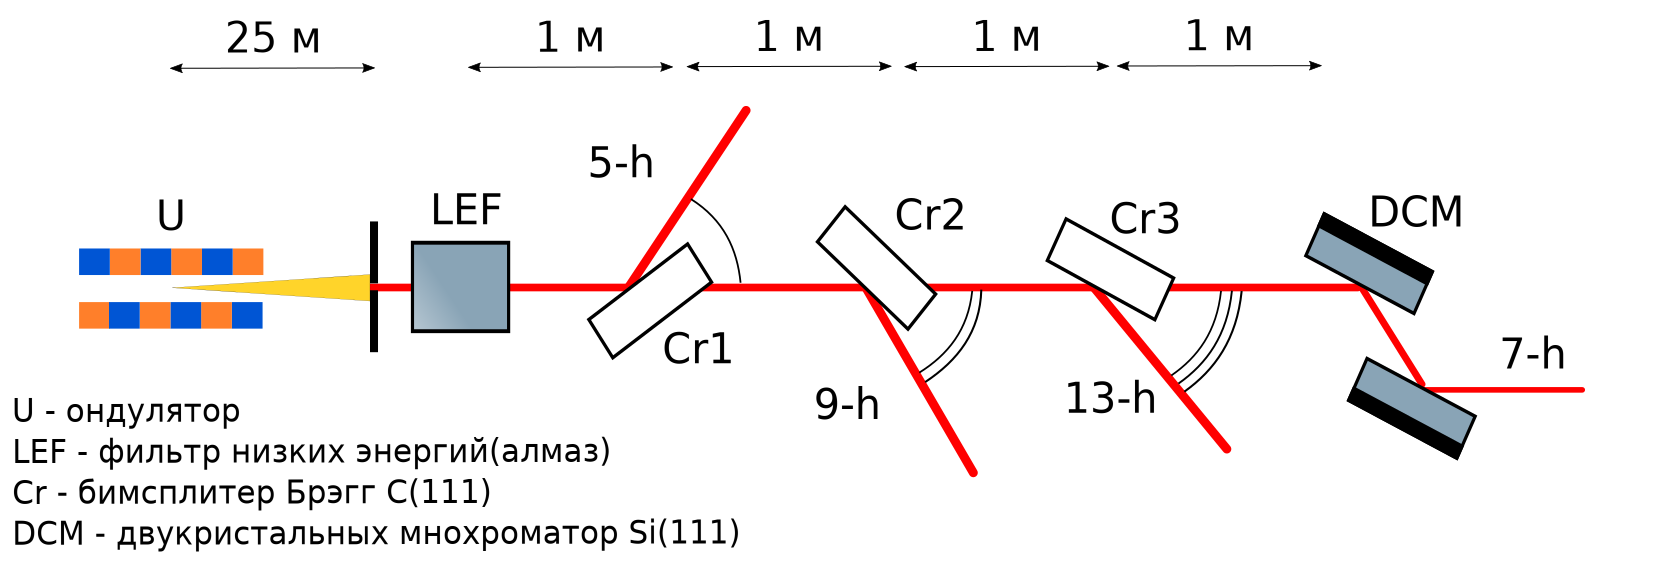
\includegraphics[width=\textwidth]{pic/OptScheme_1-2.pdf}
	\caption{Оптическая схема станции 1-2}
	\label{fig:OptScheme_1-2}  
\end{figure}
На рис.~\ref{fig:full_spec_1-2} приведены удельные тепловые нагрузки на элементы станции. Толщина кристалла алмазных бис-сплиттеров та же --- $100 \; \textup{мкм}$. Приведено сравнение удельных тепловых нагрузок на оси, результаты расчётов приведены на рис.~\ref{fig:full_spec_1-2}, с независимым методом кода SRW см.рис.~\ref{fig:power_dens_1-2}. Для~\ref{fig:full_spec_1-2} --- $74,6 \; \textup{Вт/мм}^2$, для рис.~\ref{fig:power_dens_1-2} --- это $74,9 \; \textup{Вт/мм}^2$. В параграфе ~\ref{subsection:opt_scheme_1-1} главы~\ref{chap:opt_schemes}
%Такое же как и для 1-1 сравнение результатов расчёта полной падающей удельной мощности на первый оптический элемент можно найти на рис.~\ref{fig:power_dens_1-2} в приложении к работе.

\textbf{Результаты расчётов расчётов в коде SRW для станции 1-2:}
\begin{figure}[h!]
	\centering
	\includegraphics[width=\textwidth]{pic/full_spec_1-2.pdf}
	\caption{Для станции 1-2: спектр на оси. Розовый цвет --- спектр электронного пучка с нулевым эмиттансом, падающий на алмазное окно, чёрный цвет --- спектр излучения, падающий на монохроматор}
	\label{fig:full_spec_1-2}   
\end{figure}

\DTLloaddb
[
noheader,
keys={},
headers={
	\shortstack{$n_{\textup{{\normalfont гарм}}}$},
	\shortstack{$\sigma_x, [\textup{{\normalfont мм}}]$},
	\shortstack{$\sigma_y, [\textup{{\normalfont мм}}]$},
	\shortstack{$\sigma_x, [\textup{{\normalfont мкрад}}]$},
	\shortstack{$\sigma_y, [\textup{{\normalfont мкрад}}]$}}
]
{RMS_before1-2}{tabl_1-2/RMS_before1-2.csv}
\begin{table}[h!]
	\caption{Для станции 1-2: сечение пучка на входе в первую апертуру (25 м) с учётом эмиттанса и энергетического разброса}
	\sisetup{
		parse-numbers   = false,
		table-number-alignment = right,
		table-figures-integer = 4,
		table-figures-decimal = 4,
		input-decimal-markers = .
	}
	\renewcommand*\dtlrealalign{S}
	\centering
	\DTLdisplaydb{RMS_before1-2}
	\label{table:size_obeam}
\end{table}

\DTLloaddb
[
noheader,
keys={},
headers={
	\shortstack{$n_{\textup{{\normalfont гарм}}}$},
	\shortstack{$\theta_{ \textup{{\normalfont Б}}}, \textup{{\normalfont град}}$},
	\shortstack{$d_{\textup{{\normalfont эф}}}, \textup{{\normalfont мкм}}$},
	\shortstack{$S_{\textup{{\normalfont пр}}}, \textup{{\normalfont мм}}$}}
]
{Cr_angles1-2}{tabl_1-2/Cr_angles1-2.csv}
\begin{table}[h!]
	\caption{Для станции 1-2: номер гармоники, ориентация кристалла, эффективная толщина алмазного бим-сплиттера, проекция пучка (горизонтальная) }
	\sisetup{
		parse-numbers   = false,
		table-number-alignment = right,
		table-figures-integer = 4,
		table-figures-decimal = 4,
		input-decimal-markers = .
	}
	\renewcommand*\dtlrealalign{S}
	\centering
	\DTLdisplaydb{Cr_angles1-2}
	\label{table:stable}
\end{table}

\DTLloaddb
[
noheader,
keys={},
headers={
	\shortstack{$n_{harm}$},
	\shortstack{$\sigma_x, [\textup{{\normalfont мм}}]$},
	\shortstack{$\sigma_y, [\textup{{\normalfont мм}}]$},
	\shortstack{$\sigma_x, [\textup{{\normalfont мкрад}}]$},
	\shortstack{$\sigma_y, [\textup{{\normalfont мкрад}}]$}}
]
{RMS_after1-2}{tabl_1-2/RMS_after1-2.csv}
\begin{table}[h!]
	\caption{Для станции 1-2: сечение пучка после бим-сплиттеров и монохроматора с учётом эмиттанса и энергетического разброса}
	\sisetup{
		parse-numbers   = false,
		table-number-alignment = right,
		table-figures-integer = 4,
		table-figures-decimal = 4,
		input-decimal-markers = .
	}
	\renewcommand*\dtlrealalign{S}
	\centering
	\DTLdisplaydb{RMS_after1-2}
	\label{table:size_obeam_after}
\end{table}

\DTLloaddb
[
noheader,
keys={},
headers={
	\shortstack{$n_{\textup{{\normalfont гарм}}}$},
	\shortstack{$E, \textup{{\normalfont [эВ]}}$},
	\shortstack{$\lambda, \textup{{\normalfont [нм] }}$},
	\shortstack{$\gamma/\textup{{\normalfont с}}$},
	\shortstack{$\gamma/\textup{{\normalfont с}}/0.1\%\mathnormal{bw}$},
	\shortstack{$\Delta E / E$}}
]
{ph_beam_par_after_cr1-2}{tabl_1-2/ph_beam_par_after_cr1-2.csv}
\begin{table}[h!]
	\caption{Для станции 1-2: потоки фотонов после бим-сплиттеров и монохроматора}
	\sisetup{
		parse-numbers   = false,
		table-number-alignment = right,
		table-figures-integer = 4,
		table-figures-decimal = 4,
		input-decimal-markers = .
	}
	\renewcommand*\dtlrealalign{S}
	\centering
	\DTLdisplaydb{ph_beam_par_after_cr1-2}
\end{table}
\vspace{5pt}
\newpage
\section{Станция 1-4 --- <<XAFS-спектроскопия и магнитный дихроизм>>}
\subsection{Вставное устройство}
На сверхпроводящий ондулятор станции 1-4 накладываются весьма специфичные условия, так как на этой станции планируется реализовать две техники: традиционная XAFS-спектроскопия и техника  быстрой XAFS-спектроскопии с временами порядка долей секунд (quick-EXAFS). Последняя техника требует довольно широкого спектра шириной, порядка, $1 \; \textup{кэВ}$ на энергии $ 10 \; \textup{кэВ}$ (т.е. $\Delta E / E \sim 10^{-1}$), что не может быть реализованно с помощью обычного планарного ондулятора, ширина спектра которого определяется количеством периодов ондулятора и составляет порядка: $\Delta E / E \sim 10^{-2}$. Для уширения спектра ондуляторного излучения используют так называемую технику тэйперинга, изменение магнитного поля некоторым способом: переменный зазор, изменения тока в катушках для сверхпроводящих ондуляторов, также можно менять длину периодов ондулятора вдоль траектории электронного пучка. Всё это делается для того, чтобы параметр ондуляторности менялся квадратичным образом,  $K = K_0 + \alpha \cfrac{dK}{dz}z + \beta \cfrac{d^{2}K}{dz^{2}}z^2$ (вклад квадратичного члена, обычно, мал).
\begin{table}[h!]
	\caption{Параметры ондулятора для станции 1-4}
	\centering
	\begin{tabular}{c|c|c|c|c}
		\hline\hline
		\rule{0pt}{3ex}$\mathnormal{B, [\textup{Тл}]}$ & $\mathnormal{d, [\textup{мм}]}$   & $\mathnormal{K}$   & $\mathnormal{L, [\textup{м}]}$  &  Рабочие Гармоники 1-4       \\ \hline
		\rule{0pt}{3ex}$0,65 - 1,37$   & $18$  & $1,1 - 2,3$  & $2,3 $                        		   & $3 - 13$\\
		\hline\hline
	\end{tabular}
	\label{table:und1-4}
\end{table}

Необходимо отметить, для реализации техники XAFS-спектроскопии на устройстве будет возможность производить сканирование по спектру. Магнитное поле должно меняться в широких пределах, посредствам подстройки тока в обмотках сверхпроводящего устройства. Параметры такого ондулятор см. в таб.~\ref{table:und1-4}. 

\begin{figure}[h!]
	\begin{minipage}{0.99\textwidth}
		\centering  
		\includegraphics[width=\textwidth]{pic/F_A.pdf}
		\caption{Спектр ондулятора для 1-4 с $K$ в диапазоне от $1,1 - 2,3$. Красной точкой обозначен спектр представленный на рис.~\ref{fig:spec_1-4}}
		\label{fig:F_A}  
	\end{minipage}\hfill
	
	\begin{minipage}{0.99\textwidth}
		\centering
		\includegraphics[width=\textwidth]{pic/log_spec_1-4.pdf}
		\caption{Спектр с ондулятора с $K = 2,3$ через апертуру $1 \; \textup{мм}$ в логарифмическом масштабе (сверху) и в линейном (снизу) посчитанный в коде SPECTRA с учётом эмиттанса и энергетического разброса}
		\label{fig:spec_1-4}
	\end{minipage}    
\end{figure}

Помимо этого, на  ондулятор накладывается условие перекрытия рабочих гармоник, чтобы предоставить пользователям вести непрерывное сканирование по энергии в широком диапазоне от $4 \; \textup{кэВ}$ до $40 \; \textup{кэВ}$. На рис.~\ref{fig:F_A} представлен спектр с указанными выше диапазона изменения $K$ ондулятора, показано эффективное перекрытие рабочих гармоник.

\subsection{Излучение клинообразного ондулятора}
Для решение задач быстрой  XAFS-спектроскопии была предложена схема планарного ондулятора специальной конструкции, который может доставить широкий спектр. Идея состоит в том, чтобы разбить ондулятор на несколько секций с различным магнитным полем в каждой из них, см. рис.~\ref{fig:section_und_sheme}.
\begin{figure}[h]
	\centering  
	\includegraphics[width=\textwidth]{pic/und.pdf}
	\caption{Ондулятор состоящий из малых ондуляторных секций. $dB/B = 1,5 \%$}
	\label{fig:section_und_sheme}  
\end{figure}
Такая расстановка, в первом приближении, должна была дать набор резонансов, которые сольются в один сплошной спектр. Однако, более детальное рассмотрение показало, что в зависимости от фазы электрона между сегментами, проявляются интерференционные эффекты, которые в значительной степени будут изменять форму спектра. 

Выкладки можно начать с модифицированного интеграла~\ref{eq:field_dist_in_integral}, 
\begin{equation}
\begin{array}{lcl}
\vec{\widetilde{E}}_{\bot}(z_0,  \vec{r}_{\bot 0}, \omega) =
\cfrac{\omega eA_{JJ}}{2c^2z_0}\cfrac{K}{\gamma}
\displaystyle\int\limits_{-\lambda_w N/2}^{\lambda_w N/2} dz'
\exp[iCz'] 	\vec{e}_x,
\end{array}	
\end{equation} 
Здесь, для простоты изложения, излучение рассматривается на оси, т.е. $\vec{\theta} = 0$ от электронного пучка с бесконечно малым эмиттансом. В случае секционного ондулятора коэффициент ондуляторности меняется вдоль ондулятора, поэтому $K = K_0 + n\Delta K$, и также $C = C_0 + n\Delta C$, где $n$ --- это номер секции. $\Delta {C}$ введено следующим образом:
\begin{equation}
C =k_w\cfrac{\Delta \omega}{\omega_r} = \cfrac{\Delta \omega_r}{2c\gamma}\bigg(1 + \cfrac{(K_0 + n\Delta K)^2}{2}\bigg) \approx \cfrac{\Delta \omega_r}{2c\gamma}\bigg(1 + \cfrac{K^2_0}{2}(1 + \cfrac{n\Delta K}{K_0})\bigg) = C_0 + \Delta C,
\end{equation} 
помня, что $\omega_r = 2c\widetilde{\gamma}^2k_w$.

Для определённости, будут рассматриваться пять секций, и для удобства нумерацию будем вести $-2, -1, ... , 2$. Поэтому интеграл можно переписать в виде:
\begin{equation}
\begin{array}{lcl}
\vec{\widetilde{E}}_{\bot}(z_0,  \vec{r}_{\bot 0}, \omega) =
\cfrac{\omega eA_{JJ}}{2c^2 \gamma}\cfrac{1}{z_0}
\displaystyle\sum\limits_{n =-2}^{2}(K_0 + n\Delta K)
\displaystyle\int\limits_{(2n + 1)L_s/2}^{(2n - 1)L_s/2} dz'
\exp[i(C_0 + n\Delta C)z']	\vec{e}_x,
\end{array}	
\end{equation} 
где $L_s$ --- длина одной секции, взяв интеграл, получим:
\begin{equation}
\begin{array}{lcl}
\vec{\widetilde{E}}_{\bot}(z_0,  \vec{r}_{\bot 0}, \omega) =
\cfrac{\omega eA_{JJ} L_s}{2c^2 \gamma}\cfrac{1}{z_0}
\displaystyle\sum\limits_{n =-2}^{2}(K_0 + n\Delta K)
\sinc(\hat{C}/2)e^{in({C}_0 + n\Delta {C})L_s}	\vec{e}_x.
\end{array}	
\end{equation} 
Возведя в квадрат, получим интенсивность:
\begin{equation}
\begin{array}{lcl}
{\widetilde{I}} =
\bigg(\cfrac{\omega eA_{JJ} L_s}{2c^2 \gamma z_0}\bigg)^2\bigg[
\displaystyle\sum\limits_{n =-2}^{2}(K_0 + n\Delta K)^2\sinc^2(\hat{C_0} + n\Delta \hat{C}/2) \; + \\

\displaystyle\mathop{\sum\limits_{n, m =-2}^{2}}_{n \neq m}K^2_0\bigg(1 + n\cfrac{\Delta K}{K_0} + m\cfrac{\Delta K}{K_0}\bigg)
\sinc^2(\hat{C}/2)e^{i(n-m)\hat{C}_0 + (n^2 - m^2)\Delta \hat{C}}\bigg],
\end{array}	
\end{equation} 
\begin{figure}[h!]
	\centering  
	\begin{minipage}{0.49\textwidth}
		\centering
		\includegraphics[width=\textwidth]{pic/spec_from_sec_und.pdf}
		\caption{Аналитический результат для электронного пучка с бесконечно малым эмиттансом}
		\label{fig:section_und_analitics}
	\end{minipage}\hfill
	\begin{minipage}{0.51\textwidth}
		\centering
		\includegraphics[width=\textwidth]{pic/sim_und_spec_new.pdf}
		\caption{Симуляция в коде SRW для электронного пучка с бесконечно малым эмиттансом}
		\label{fig:section_und_SRW}
	\end{minipage}    
\end{figure}
Полученное выражение можно проинтерпретировать следующим образом: первая сумма --- есть сумма сдвинутых по соответствующим резонансам $\sinc^2$ функций, вторая сумма отображает интерференцию между различными секциями ондулятора. Данная комбинация приводит к колебаниями в спектре, как показано на рис.~\ref{fig:section_und_analitics} синими пунктирными линиями при значении параметра $\Delta C = 6$, чёрной пунктирной линией отмечена сумма $\sinc^2$ функций без учёта интерференционных слагаемых.

\begin{figure}[h!]
	\centering  
	\includegraphics[width=0.6\textwidth]{pic/sim_und_spec_new_mm.pdf}
	\caption{Спектр секционного ондулятора проинтегрированного по конечной апертуре --- $1 \; \textup{мм}$ с учётом эмиттанса и энергетического разброса}
	\label{fig:sim_und_spec_new_mm}  
\end{figure}

На рис.~\ref{fig:section_und_SRW} показан характерный спектр секционного ондулятора посчитанного при помощи симуляционного кода SRW. Сравнивая рис.~\ref{fig:section_und_SRW} и~\ref{fig:section_und_analitics} можно сделать вывод, что характер спектра в численном моделировании совпадает с характером спектра в используемом аналитическом приближении.  На рис.~\ref{fig:sim_und_spec_new_mm} представлен спектр с учётом эмиттанса и энергетического разброса в пучке, проинтегрированный по конечной апертуре --- $1 \; \textup{мм}$ на расстоянии $22 \; \textup{м}$.

\subsection{Оптика станции 1-4}

На рис.~\ref{fig:OptScheme_1-4} представлена оптическая схема станции для реализации XAFS-спектроскопии, которая состоит из двуxкристального монохроматора и системы зеркал Киркпатрика-Баеза для фокусировки излучения на образец. Для реализации быстрой XAFS-спектроскопии будет использоваться отдельный монохроматор, однако, в данной работе оптическая схема для указанного метода рассматриваться не будет.

\begin{figure}[h]
	\begin{minipage}{0.99\textwidth}
	\centering  
	\includegraphics[width=\textwidth]{pic/OptScheme_1-4.pdf}
	\end{minipage}\hfill
	\begin{minipage}{0.3\textwidth}
		\centering
		\includegraphics[width=\textwidth]{pic/3_harm_before_optics_2d.pdf}
%		\caption{Сечение пучка до апертуры}
%		\label{fig:3_harm_before_optics_2d}
	\end{minipage}
	\begin{minipage}{0.3\textwidth}
		\centering
		\includegraphics[width=\textwidth]{pic/3_harm_after_DCM_2d.pdf}
%		\caption{Сечение пучка после DCM}
%		\label{fig:3_harm_after_DCM_2d}
	\end{minipage} 
	\begin{minipage}{0.3\textwidth}
		\centering
		\includegraphics[width=\textwidth]{pic/3_harm_after_Sph_Mir_2d.pdf}
%		\caption{Сечение пучка около фокуса зеркал}
%		\label{fig:3_harm_after_Sph_Mir_2d}
	\end{minipage} 
	\caption{Оптическая схема станции 1-4. Ниже сечения пучка слева на право: на выходе апертуры, на выходе после двухкритального монохроматора, на выходе после фокусирующих зеркал}
	\label{fig:OptScheme_1-4}  
\end{figure}
